\documentclass[11pt,a4paper]{article}

\usepackage[margin=1in, paperwidth=8.3in, paperheight=11.7in]{geometry}
\usepackage{amsfonts}
\usepackage{amsmath}
\usepackage{amssymb}
\usepackage{color}
\usepackage{enumerate}
\usepackage{enumitem}
\usepackage{fancyhdr}
\usepackage[none]{hyphenat}  % Don't hyphen break words at line breaks
\usepackage[latin1]{inputenc}
\usepackage{stmaryrd}
\usepackage{tikz}
\usetikzlibrary{shapes,arrows,positioning}

\begin{document}

\pagestyle{fancy}
\setlength\parindent{0pt}
\allowdisplaybreaks

% Counters
\newcounter{definition}[section]
\newcounter{example}[section]
\newcounter{notation}[section]
\newcounter{proposition}[section]
\newcounter{remark}[section]
\newcounter{theorem}[section]

% enumerate uses roman
\setlist[enumerate,1]{label=\roman*)}

% commands
\newcommand{\eg}{\textit{e.g.} }
\newcommand{\EG}{\underline{E.G.} - }
\newcommand{\ie}{\textit{i.e.} }
\newcommand{\IE}{\underline{I.E.} - }
\newcommand{\NB}{\underline{N.B.} - }
\newcommand{\nats}{\mathbb{N}}
\newcommand{\reals}{\mathbb{R}}
\newcommand{\binomial}[2]{{{#1}\choose{#2}}}
\newcommand{\Binomial}[2]{\displaystyle{{{#1}\choose{#2}}}}
\newcommand\doubleplus{+\kern-1.3ex+\kern0.8ex} % ++

\newcommand{\notation}[1]{\stepcounter{notation} \textbf{Notation \arabic{section}.\arabic{notation}\ - }\textit{#1}\\}
\newcommand{\proof}[1]{\stepcounter{proof} \textbf{Proof \arabic{section}.\arabic{proof}\ - }\textit{#1}\\}
\newcommand{\proposition}[1]{\stepcounter{proposition} \textbf{Proposition \arabic{section}.\arabic{proposition}\ - }\textit{#1}\\}
\newcommand{\Proposition}[1]{\stepcounter{proposition} \textbf{Proposition \arabic{section}.\arabic{proposition}\ - }\textit{#1}}
\newcommand{\theorem}[1]{\stepcounter{theorem} \textbf{Theorem \arabic{section}.\arabic{theorem}\ - }\textit{#1}\\}
\newcommand{\definition}[1]{\stepcounter{definition} \textbf{Definition \arabic{section}.\arabic{definition}\ - }\textit{#1}\\}
\newcommand{\example}[1]{\stepcounter{example} \textbf{Example \arabic{section}.\arabic{example}\ - }\textit{#1}\\}

% enviroments
\renewcommand{\headrulewidth}{0pt}

% Cover page title
\title{Combinatorics - Reviewed Notes}
\author{Dom Hutchinson}
\date{\today}
\maketitle

% Header
\fancyhead[L]{Dom Hutchinson}
\fancyhead[C]{Combinatorics - Reviewed Notes}
\fancyhead[R]{\today}

\tableofcontents
\newpage

\section{Counting Techniques}

\theorem{Bijection Rule}
A set $X$ has $n\in\nats$ elements iff $\exists$ a bijection $f:X\to[n]$.\\

\theorem{Addition Rule}
Let $A_1,\dots,A_n$ be finite pairwise disjoint sets. Then
$$\left|\bigcup_{i=1}^nA_i\right|=\sum_{i=1}^n|A_i|$$

\theorem{Multiplication Rule}
If a counting problem can be split into $n$ independent stages, each of which involves choosing an option out of a set $A_i$. Then the total number of possible outcomes is
$$\mathrm{Possible\ Outcomes}=\prod_{i=1}^n|A_i|$$

\theorem{Inclusion-Exclusion Principle}
Let $A_1,\dots,A_n$ be finite sets. Then
$$\left|\bigcup_{i=1}^nA_i\right|=\sum_{i=1}^n|A_i|-\sum_{i_1<i_2}|A_{i_1}\cap A_{i_2}|+\sum_{i_1<i_2<i_3}|A_{i_1}\cap A_{i_2}\cap A_{i_3}|-\dots+(-1)^{n+1}|A_1\cap\dots\cap A_n|$$

\theorem{Binomial Coefficient Identities}
\[\begin{array}{cc}
\Binomial{n}{k}=\Binomial{n}{n-k},&\Binomial{n}{0}=1=\Binomial{n}{n}\\
\Binomial{n}{k}=0\ \forall\ k>n,&\Binomial{n}{k}=\dfrac{(n)_k}{k!}=\dfrac{n!}{k!(n-k)!}
\end{array}\]

\definition{Ordered Selection}
In an \textit{Ordered Selection} problem we are selecting $k$ elements from a set of $n$, and care about the order in which we pick them, so $\{x_1,x_2\}\not\equiv\{x_2,x_1\}$.\\

\definition{Unordered Selection}
In an \textit{Unordered Selection} problem we are selecting $k$ elements from a set of $n$, and do not care about the order we pick them so $\{x_1,x_2\}\equiv\{x_2,x_1\}$.\\

\proposition{Number of Possible Selections}
The table below summarises the number of possible ways to choose $k$ elements from a set of $n$, for each scenario of selection problems.\\
\begin{tabular}{|c|c|c|}
\hline
&Ordered Selection&Unordered Selection\\
\hline
With Repetition&$n^k$&$\Binomial{n+k-1}{k}$\\
\hline
Without Repetition&$\dfrac{n!}{(n-k)!}$&$\Binomial{n}{k}$\\
\hline
\end{tabular}\\

\theorem{Pascal's Identity}
$$\binomial{n}{i}=\binomial{n-1}{i}+\binomial{n-1}{i-1}\ \forall\ i\in\nats^{\leq n}$$

\theorem{Binomial Theorem}
$$(a+b)^n=\sum_{i=0}^n\binomial{n}{i}a^ib^{n-i}\ \forall\ a,b\in\reals\ n\in\nats$$

\theorem{Sum of Binomial Coefficients}
$$\sum_{i=0}^n\Binomial{n}{i}=2^n$$

\theorem{Identity}
$$(j+1)\Binomial{n}{j+1}=n\Binomial{n-1}{j}$$

\theorem{Pigeonhole Principle}
If there are more pigeons than pigeonholes, then at least $2$ pigeons must occupy the same hole.\\

\theorem{Generalised Pigeonhole Principle}
If $m$ objects are distributed into $n$ boxes and $m>nk$ for $k\in\nats$, then at least one box contains at least $k+1$ objects.

\section{Generating Functions}

\definition{Generating Functions}
Given a sequence $(a_n)_{n\geq0}$ with $a_i\in\reals$ we associate the power series $f(x)=\sum_{i=0}^\infty a_nx^n$.\\
$f(x)$ is the \textit{Generating Function} of the sequence $(a_n)_{n\geq0}$.\\

\theorem{Scaling Rule}
$$\mathrm{If}\ f(x)\leftrightarrows(a_0,a_1,a_2,\dots)\implies cf(x)\leftrightarrows(ca_0,ca_1,ca_2,\dots)$$

\theorem{Addition Rule}
$$\mathrm{If}\ f(x)\leftrightarrows(a_0,a_1,a_2,\dots)\ \&\ g(x)\leftrightarrows(b_0,b_1,b_2,\dots)\implies f(x)+g(x)\leftrightarrows (a_0+b_0,a_1+b_1,\dots)$$

\theorem{Right Shift Rule}
$$\mathrm{If}\ f(x)\leftrightarrows(a_0,a_1,a_2,\dots)\implies x^kf(x)\leftrightarrows(\underbrace{0,\dots,0}_{k\ \mathrm{times}},a_0,a_1,a_2,\dots)$$

\theorem{Differentiation Rule}
$$\mathrm{If}\ f(x)=\sum_{i=0}^\infty a_ix^i\leftrightarrows(a_0,a_1,a_2,\dots)\implies f'(x)=\sum_{i=0}^\infty ia_{i+1}x^i\leftrightarrows(a_1,2a_2,3a_3,\dots)$$

\theorem{Convolution Rule}
$$\mathrm{If}\ f(x)\leftrightarrows(a_0,a_1,a_2,\dots)\ \& \ g(x)\leftrightarrows(b_0,b_1,b_2,\dots)\implies f(x)\cdot g(x)\leftrightarrows(c_0,c_1,c_2,\dots)\ \mathrm{where}\ c_i:=\sum_{j=0}^ia_jb_{i-j}$$

\definition{Recurrence Relation}
A sequence, $(a_n)_{n\geq0}$ is a \textit{Recurrence Relation} if, for large enough $n$, $a_n$ is defined in terms of its previous terms. Generating functions can be used to express $(a_n)_{n\geq0}$ in terms of $n$.\\

\theorem{Generating Function Identities}
\[\begin{array}{rcl}
\dfrac{1}{1-x}&\leftrightarrows&(1,1,1,\dots)\\
(1+x)^n&\leftrightarrows&\left(\Binomial{n}{k}\right)_{k\geq0}\\
(1+x)^{-n}&\leftrightarrows&\displaystyle{\sum_{i=0}^\infty(-1)^k\Binomial{n+k-1}{k}x^k}\\
\end{array}\]

\theorem{Sum Identities}
\[\begin{array}{rcl}
\displaystyle{\left(\sum_{i=0}^\infty x^i\right)^n}&=&\displaystyle{\sum_{i=0}^\infty\Binomial{n+k-1}{k}x^k}\\
\dfrac{1}{(1-x)^n}&=&\displaystyle{\sum_{i=0}^\infty\Binomial{n+k-1}{k}x^k}
\end{array}\]

\section{Combinatorial Design}

\definition{Set System}
$(V,\mathcal{B})$ is a \textit{Set System} where $V$ is a finite set \& $\mathcal{B}$ is a set of subsets, which are not necessarily disjoint), of $V$. $V$ is called the \textit{Ground Set} \& $\mathcal{B}$ is called \textit{Blocks}.\\

\definition{$k$-Uniform}
A \textit{Set System}, $(V,\mathcal{B})$, is $k$-uniform iff $\forall\ B\in\mathcal{B},\ |B|=k$.\\

\definition{Block Design}
Let $v,k,t,\lambda\in\nats$ with $v>k\geq k\geq t\geq 1$.\\
A \textit{Block Design} of type $t-(v,k,\lambda)$ is a set system $(V,\mathcal{B})$ with
\begin{itemize}
	\item[-] $|V|=v$;
	\item[-] $\forall\ B\in\mathcal{B},\ |B|=k$; and,
	\item[-] $\forall\ T\subseteq V$ with $|T|=t\ \exists\ \lambda$ blocks, $B\in\mathcal{B}$, with $T\subseteq B$.
\end{itemize}

\definition{Fano Plane}
The \textit{Fano Plane} is a set-system with  $V=\{1,2,3,4,5,6,7\}$\\
\& $\mathcal{B}=\{\{1,2,3\},\{1,4,7\},\{3,6,7\},\{1,5,6\},\{3,4,5\},\{2,5,7\},\{2,4,6\}\}$. This is a \textit{Block Design} of type $2-(7,3,1)$.\\
\includegraphics[scale=0.25]{img/fanoplane.png}\\
\NB This is the smallest example of a \textit{Finite Projective Plane}.\\

\definition{Replication Number}
The \textit{Replication Number} is the number of blocks each element appears in in a \textit{Block Design}.\\

\theorem{Number of Blocks in Block Design}
The number of blocks in a block design of type $t-(v,k,\lambda)$ is found by the following formula
$$b:=\frac{\lambda\binomial{v}{t}}{\binomial{k}{t}}$$

\theorem{Replication Number}
In a block design of type $2-(v,k,\lambda)$ every element lies in $r$ blocks where
$$r:=\frac{(k-1)}{\lambda(v-1)}=\frac{bk}{v}$$

\theorem{Fisher's Inequality}
Let $(V,\mathcal{B})$ be a block design of type $2-(v,k,\lambda)$ with $v>k$. Then$$|\mathcal{B}|\geq|V|$$

\definition{Incidence Matrix}
The \textit{Incidence Matrix} of a \textit{Set System} $(V,\mathcal{B})$ is a $|V|\times|\mathcal{B}|$ matrix where
$$a_{i,j}=\begin{cases}1&\mathrm{if}\ v_i\in B_j\\0&\mathrm{otherwise}\end{cases}$$

\section{Graph Theory}

\subsection{Introduction}

\definition{Graph}
A \textit{Graph}, $G$, is an ordered pair $(V,E)$ where $V$ is a set of vertices \& $E$ is a set of edges between these vertices. Edges are represented by a $2$-element subset of $V$.\\

\definition{Sub-Graph}
Consider a graph $G=(V,E)$. $G'=(V',E')$ is a \textit{Sub-Graph} of $G$ if
$$V'\subseteq V\ \&\ E'=\{\{u,v\}\in E:u,v\in V'\}$$

\definition{Induced Sub-Graph}
A \textit{Sub-Graph} $G'=(V',E')$ of $G=(V,E)$ is an \textit{Induced Sub-Graph} if $E'$ contains all the edges in $E$ that run between vertices in $V'$.\\

\definition{Order of a Graph}
The \textit{Order} of a \textit{Graph} $G=(V,E)$ is the number of vertices, $|V|$.\\

\definition{Simple Graph}
A \textit{Simple Graph} is an unweighted, undirected with no edges which start \& end on the same vertex, nor duplicate edges.\\

\proposition{Graphs are $2$-Uniform Set Systems}

\definition{Adjacency}
For a graph $G=(V,E)$, $u,v\in V$ are \textit{Adjacent} if $\{u,v\}\in E$.\\

\definition{Neighbourhood}
Consider a graph $G=(V,E)$ \& $v\in V$. The \textit{Neighbourhood} of $v$ in $G$ is the vertices adjacent to $v$ in $G$.
$$N_G(v):=\big\{u:u\in V\ \&\ \{u,v\}\in E\big\}$$

\definition{Neighbourhood of a Set of Vertices}
Let $G=(V,E)$ be a graph, then for $S\subseteq V$
$$N_G(S):=\bigcup_{s\in S}N_G(s)$$

\definition{Degree}
Consider a graph $G=(V,E)$ \& $v\in V$. The \textit{Degree} of $v$ is the size of its \textit{Neighbourhood} of $v$.
$$deg_G(v):=|N_G(v)|$$

\theorem{Handshaking Lemma}
Consider a graph $G=(V,E)$. Then
$$|E|=\frac{1}{2}\sum_{v\in V}deg_G(v)$$

\theorem{Maximum Number of Edges}
A graph has at most $\Binomial{n}{2}=\frac{1}{2}n(n-1)$ edges.

\definition{Graph Isomorphism}
Two graphs $G_1=(V_1,E_1)$ \& $G_2=(V_2,E_2)$ are \textit{Isomorphic} if $\exists$ a bijection $\phi:V_1\to V_2$ st
$$\forall\ \{u,v\}\in E_1\implies \{\phi(u),\phi(v)\}\in E_2$$

\definition{Degree Sequence}
Consider a graph $G=(V,E)$. Order the vertices $\{v_1,\dots,v_n\}$ with $deg(v_i)\leq deg(v_j)\ \forall\ i<j$. The \textit{Degree Sequence} of $G$ is
$$\big(deg(v_1),\dots,deg(v_n)\big)$$

\theorem{Isomorphic Graphs}
If two graphs are isomorphic then the following properties hold
\begin{enumerate}
	\item They have the same number of edges;
	\item They have the same \textit{Degree Sequence}.
\end{enumerate}

\subsection{Types of Graph}

\definition{Walk}
Consider a graph $G=(V,E)$ and $u,v\in V$. A \textit{Walk} from $u$ to $v$ is a sequence of not-necessarily-distinct vertices $V_c=(u=x_1,x_2,\dots,x_n=v)$ with $E_c=\big\{\{x_i,x_{i+1}\}:i\in[1,n-1]\big\}\subseteq E$. Neither the edges, nor vertices, are necessarily unique.\\

\definition{Circuit}
A \textit{Circuit} is a closed \textit{Walk}.\\
\NB A \textit{Circuit} is generally not a graph since they often have repeated edges.\\

\definition{Trail}
A \textit{Trail} is a \textit{Walk} with no repeated edges. It can still have repeated vertices.\\

\definition{Path}
A \textit{Path} of length $n$ has vertex set $V_P=\{v_1,\dots,v_n:v_i\neq v_j\ \forall\ i\neq j\}$ \& edge set $E_p=\{\{v_i,v_{i+1}\}:i\in[1,n-1]\}\subseteq E$. All vertices, and thus edges, in a path are distinct.\\

\definition{Connected}
Two vertices are \textit{Connected} if there exists a path between them.\\
A \textit{Graph} is \textit{Connected} if there exists a path between all pairs of vertices in it.\\

\definition{Disconnected}
A \textit{Graph} $G=(V,E)$ is \textit{Disconnected} if there $\exists\ u,v\in V\ st\ \nexists$ a path in $G$ between $u$ \& $v$. The \textit{Maximally Connected Sub-Graphs} of $G$ are called \textit{Components} of $G$.\\

\definition{Cycle}
A \textit{Cycle} of length $n$ has vertex set $V_c=\{v_1,\dots,v_n:v_i\neq v_j\ \forall\ i\neq j\}$ \& edge set $E_c=\{v_n,v_1\}\cup\big\{\{v_i,v_j\}:i\in[1,n-1]\}\big\}$. This is a path that starts and ends on the same vertex.\\

\theorem{If a graph admits an odd circuit, then it admits an odd cycle}

\definition{Tree}
A \textit{Tree} is a \textit{Graph} with no cycles.\\

\definition{Star}
A \textit{Star} is a \textit{Graph} $G=(V,E)$ with $V=\{v_1,\dots,v_n\}$ \& $E=\{\{v_1,v_i\}:i\in[2,n]\}$.\\

\definition{Complete Graph}
A \textit{Complete Graph} is a \textit{Graph} $G=(V,E)$ with $V=\{v_1,\dots,v_n\}$ \& $E=\{\{v_i,v_j\}:i\neq j\}$. There exists an edge between each pair of vertices.\\

\example{Common Graphs}
\begin{tabular}{|l|l|l|l|}
\hline
Path, $P_4$&\begin{tikzpicture}[baseline=(current bounding box.center)]
	\node[shape=circle] (1) at (0,0) {$x_1$};
	\node[shape=circle] (2) at (1,2) {$x_2$};
	\node[shape=circle] (3) at (2,0) {$x_3$};
	\node[shape=circle] (4) at (3,2) {$x_4$};
	\node[shape=circle] (5) at (4,0) {$x_5$};
	
	\path [-] (1) edge (2);
	\path [-] (2) edge (3);
	\path [-] (3) edge (4);
	\path [-] (4) edge (5);
\end{tikzpicture}&
Disconnected&\begin{tikzpicture}[baseline=(current bounding box.center)]
	\node[shape=circle] (1) at (0,0) {$x_1$};
	\node[shape=circle] (2) at (1,2) {$x_2$};
	\node[shape=circle] (3) at (2,0) {$x_3$};
	\node[shape=circle] (4) at (4,2) {$x_4$};
	\node[shape=circle] (5) at (4,0) {$x_5$};
	
	\path [-] (1) edge (2);
	\path [-] (2) edge (3);
	\path [-] (1) edge (3);
	\path [-] (5) edge (4);
\end{tikzpicture}\\\hline
Wal \& Trail&\begin{tikzpicture}[baseline=(current bounding box.center)]
	\node[shape=circle] (1) at (0,0) {1};
	\node[shape=circle] (2) at (2,0) {2};
	\node[shape=circle] (3) at (4,0) {3};
	\node[shape=circle] (4) at (4,-2) {4};
	
	\path [->] (1) edge (2);
	\path [->] (2) edge (3);
	\path [->] (4) edge (2);
	\path [->] (4) edge (3);
\end{tikzpicture}&
Cycle, $C_5$&\begin{tikzpicture}[baseline=(current bounding box.center)]
	\node[shape=circle] (1) at (0,0) {$x_1$};
	\node[shape=circle] (2) at (1,2) {$x_2$};
	\node[shape=circle] (3) at (2,1) {$x_3$};
	\node[shape=circle] (4) at (3,2) {$x_4$};
	\node[shape=circle] (5) at (4,0) {$x_5$};
	
	\path [-] (1) edge (2);
	\path [-] (2) edge (3);
	\path [-] (3) edge (4);
	\path [-] (4) edge (5);
	\path [-] (5) edge (1);	
\end{tikzpicture}\\\hline
Tree&\begin{tikzpicture}[baseline=(current bounding box.center)]
	\node[shape=circle] (1) at (0,0) {$x_1$};
	\node[shape=circle] (2) at (-1,-1) {$x_2$};
	\node[shape=circle] (3) at (0,-1) {$x_3$};
	\node[shape=circle] (4) at (1,-1) {$x_4$};
	\node[shape=circle] (5) at (0,-2) {$x_5$};
	\node[shape=circle] (6) at (2,-2) {$x_6$};
	
	\path [-] (1) edge (2);
	\path [-] (1) edge (3);
	\path [-] (1) edge (4);
	\path [-] (4) edge (5);
	\path [-] (4) edge (6);	
\end{tikzpicture}&
Star&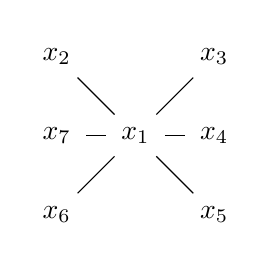
\begin{tikzpicture}[baseline=(current bounding box.center)]
	\node[shape=circle] (1) at (0,0) {$x_1$};
	\node[shape=circle] (2) at (-1,1) {$x_2$};
	\node[shape=circle] (3) at (1,1) {$x_3$};
	\node[shape=circle] (4) at (1,0) {$x_4$};
	\node[shape=circle] (5) at (1,-1) {$x_5$};
	\node[shape=circle] (6) at (-1,-1) {$x_6$};
	\node[shape=circle] (7) at (-1,0) {$x_7$};
	
	\path [-] (1) edge (2);
	\path [-] (1) edge (3);
	\path [-] (1) edge (4);
	\path [-] (1) edge (5);
	\path [-] (1) edge (6);	
	\path [-] (1) edge (7);	
\end{tikzpicture}\\\hline
Complete, $K_4$&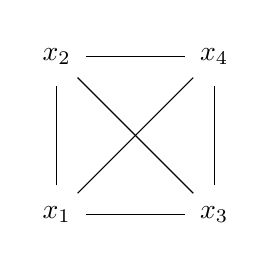
\begin{tikzpicture}[baseline=(current bounding box.center)]
	\node[shape=circle] (1) at (0,0) {$x_1$};
	\node[shape=circle] (2) at (0,2) {$x_2$};
	\node[shape=circle] (3) at (2,0) {$x_3$};
	\node[shape=circle] (4) at (2,2) {$x_4$};
	
	\path [-] (1) edge (2);
	\path [-] (1) edge (3);
	\path [-] (1) edge (4);
	\path [-] (2) edge (3);
	\path [-] (2) edge (4);
	\path [-] (3) edge (4);
\end{tikzpicture}
\\\cline{1-2}
\end{tabular}\\

\definition{Eulerian Circuit}
An \textit{Eulerian Circuit} is a \textit{Circuit} that traverses every edge exactly once. It traverses every edge exactly once, with no repeated vertices.\\
\NB A \textit{Eulerian Graph} admits an \textit{Eulerian Circuit}.\\

\theorem{Every vertex of a connected graph has even degree $\Leftrightarrow$ Eulerian Graph}

\theorem{Decomposing into Cycles}
If every vertex of a graph has even degree then its edge set can be partitioned into disjoint subsets st each subset is a cycle.\\

\definition{Hamiltonian Path}
A \textit{Hamiltonian Path} is a path that visits every vertex.\\

\definition{Hamiltonian Cycle}
A \textit{Hamiltonian Cycle} is a cycle that visits every vertex in a graph.\\
\NB A \textit{Hamiltonian Graph} admits a \textit{Hamiltonian Cycle}.\\

\theorem{Dirac's Theorem}
Let $G$ be a graph of order $n\geq 3$. If $\delta(G)\geq\frac{n}{2}$ then $G$ is \textit{Hamiltonian}.\\

\definition{$k$-Partite Graph}
Consider a graph $G=(V,E)$, $G$ is a \textit{$k$-Partite Graph} if $V$ can be partitioned into $k$ disjoint vertex classes, $\{V_1,\dots,V_k\}$, st $E\subseteq\{\{x,y\}:x\in V_i,\ y\in V_j,\ i\neq j\}$.\\

\definition{Complete $k$-Partite Graph}
A $k$-Partite Graph, $G=(V,E)$ with vertex classes $\{V_1,\dots,V_k\}$, is a \textit{Complete $k$-Partite Graph} if $E=\{\{x,y\}:x\in V_i,\ y\in V_j,\ i\neq j\}$.\\

\definition{Bipartite Graph}
A graph $G=(V,E)$ is a \textit{Bipartite Graph} iff $V$ can be partitioned into two sets $V_1$ \& $V_2$ st $V_1\cup V_2=V$, $V_1\cap V_2=\emptyset$ \& $\forall\ u\in V_1,\ v\in V_2\ \{u,v\}\not\in E$.\\
\NB - This graph is denoted $G=(V_1\cup V_2,E)$.\\

\theorem{Characterisation of Bipartite Graph}
A graph is bipartite iff it contains no odd cycles.\\

\theorem{Handshaking Lemma for Bipartite Graph}
Let $G=(V_1\cup V_2,E)$ be a bipartite graph. Then
$$\sum_{v\in V_1}deg_G(v)=\sum_{u\in V_2}deg_G(u)$$

\definition{Matching}
Consider a bipartite graph $G=(X\cup Y,E)$ a \textit{Matching} from $X$ to $Y$ is a set of edges $\{\{x,y\}:x\in X,y\in Y\}$ where no two edges have a vertex in common.\\

\theorem{Hall's Theorem}
Consider a bipartite graph $G=(X\cup Y,E)$. Then
$$\exists\ \mathrm{matching\ from}\ X\ \mathrm{to}\ Y\Leftrightarrow\ \forall\ s\subseteq X,|N_G(S)|\geq|S|$$

\theorem{Degree Constrained Version of Hall's Theorem}
Consider a bipartite graph $G=(X\cup Y,E)$. Then
$$\delta(X)\geq\Delta(Y)\Leftrightarrow\exists\ \mathrm{matching\ from}\ X\ \mathrm{to}\ Y$$

\subsection{Trees \& Forests}

\definition{Acyclic}
A graph is \textit{Acyclic} if it contains \underline{no} cycles.\\
\NB An \textit{Acyclic Graph} is called a \textit{Forest}.\\

\proposition{A tree is an acyclic connected graph}

\definition{Leaf}
A vertex of degree one is called a \textit{Leaf}.\\

\theorem{Every tree on at least two vertices has a leaf}

\theorem{Characterisation of Trees}
The following are different ways to characterise a tree $G=(V,E)$
\begin{enumerate}
	\item $G$ is maximally acyclic (\ie $G$ is acyclic \& any additional edge creates a cycle).
	\item $G$ is minimally collected (\ie $G$ is connected \& the removal of any edge disconnects $G$).
	\item $G$ is connected and $|E|=|V|-1$.
	\item $G$ is acyclic and $|E|=|V|-1$.
	\item Any two vertices in $G$ has a unique path.
\end{enumerate} 

\definition{Spanning Tree}
Consider a graph $G=(V,E)$, any tree on all vertices in $V$ is a \textit{Spanning Tree}.\\
\NB$T=(V,E')$ with $E'\subseteq E$.\\

\example{Spanning Tree}
Below is a graph and then a spanning tree of that graph\\
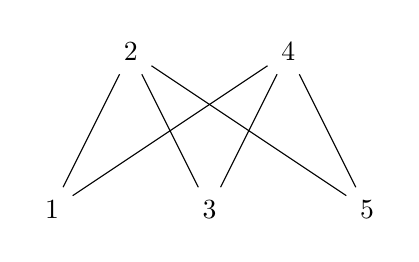
\begin{tikzpicture}
	\node[shape=circle] (1) at (0,0) {1};
	\node[shape=circle] (2) at (1,2) {2};
	\node[shape=circle] (3) at (2,0) {3};
	\node[shape=circle] (4) at (3,2) {4};
	\node[shape=circle] (5) at (4,0) {5};
	
	\path [-]
	(1) edge (2)
	(1) edge (4)
	(3) edge (2)
	(3) edge (4)
	(5) edge (2)
	(5) edge (4);
\end{tikzpicture}
\begin{tikzpicture}
	\node[shape=circle] (1) at (0,0) {1};
	\node[shape=circle] (2) at (1,2) {2};
	\node[shape=circle] (3) at (2,0) {3};
	\node[shape=circle] (4) at (3,2) {4};
	\node[shape=circle] (5) at (4,0) {5};
	
	\path [-]
	(1) edge (2)
	(1) edge (4)
	(3) edge (2)
	(5) edge (4);
\end{tikzpicture}

\theorem{Every connected graph contains a spanning tree}

\definition{Weight Function}
For $G=(V,E)$ we define a \textit{Weight Function} $W:V\to\reals$.\\

\definition{Minimum Spanning Tree}
Consider a graph $G=(V,E)$ with a weight function $W:V\to\reals$. Let $T$ be a \textit{Spanning Tree} of $G$. $T=(V,E')$ is a \textit{Minimum Spanning Tree} if $W(E'):=\sum_{e\in E'}W(e)$ is minimised relative to the other \textit{Spanning Tree}s of $G$.\\

\theorem{Algorithm for Finding Spanning Tree}
Let $G=(V,E)$ be a graph with $n$ vertices and $m$ edges.\\
Order the edges of $G$ arbitrarily into a sequence $e_1,\dots,e_m$.\\
The algorithm constructs sets of edges $E_0,E_1,\dots,\subseteq E$ in stances.\\
Set $E_0=\emptyset$.\\
At state $i$ the algorithm has already defined $E_{i-1}$. Then
$$E_i=\begin{cases}E_{i-1}\bigcup\{e_i\}&\mathrm{If\ graph\ }(V,E_{i-1}\bigcup\{e_i\}\ \mathrm{contains\ no\ cycles}\\E_{i-1}&\mathrm{otherwise}\end{cases}$$
The algorithm stops if after stage $i$ we have that$|E_i|=n-1$.\\
This condition means that $(V,E_i)$ is a tree.\\

\theorem{Kruskal's Algorithm}
Let $G=(V,E)$ be a connected weighted graph equipped with weight function $W:E\to\reals$.\\
Label the edges of $G$ with $e_1,\dots,e_m$, with $m=|E|$, in such a way that
$$W(e_1)\leq\dots\leq W(e_m)$$
Set $E_0=\emptyset$.\\
At state $i$ the algorithm has already defined $E_{i-1}$. Then
$$E_i=\begin{cases}E_{i-1}\bigcup\{e_i\}&\mathrm{If\ graph\ }(V,E_{i-1}\bigcup\{e_i\}\ \mathrm{contains\ no\ cycles}\\E_{i-1}&\mathrm{otherwise}\end{cases}$$
The algorithm stops if after stage $i$ we have that$|E_i|=n-1$.\\
\NB This is the algorithm from \textbf{Definition 6.6}.\\

\subsection{Cliques}

\definition{$k$-Clique}
A \textit{$k$-Clique} is a sub-graph which is a \textit{Complete Graph} on $k$ vertices.\\

\theorem{Mantel's Theorem}
Consider a graph $G=(V,E)$, with $n:=|V|$, containing no $3$-cycle sub-graphs. Then
\begin{enumerate}
	\item $|E|\leq\lfloor\frac{n^2}{4}\rfloor$; \&
	\item $\exists$ a graph where $|E|=\lfloor\frac{n^2}{4}\rfloor$.
\end{enumerate}
\NB The graph described $ii)$ is isomorphic to $K_{\lfloor n/2\rfloor,n-\lfloor n/2\rfloor}$.\\

\definition{Tur\'an Graph}
A \textit{Tur\'an Graph} is a graph $T_k(n)$ that is a  \textit{Complete $k$-Partite Graph} on $n$ vertices with vertex classes $\{V_1,\dots,V_k\}$ where the difference in size of any pair of vertices is no more than $1$ (\ie $\big||V_i|-|V_j|\big|\leq1\ \forall\ i,j\in[1,k]$).\\

\example{Turan Graph, $T_3(7)$}
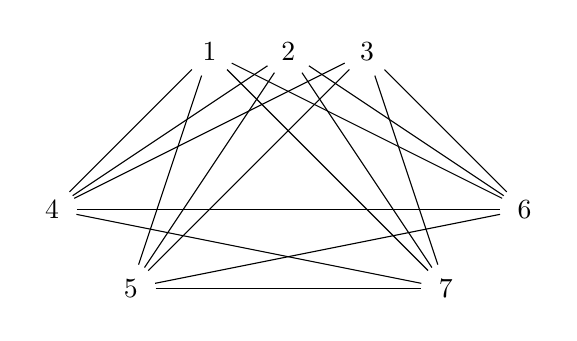
\begin{tikzpicture}
	\node[shape=circle] (1) at (0,0) {1};
	\node[shape=circle] (2) at (1,0) {2};
	\node[shape=circle] (3) at (2,0) {3};
	\node[shape=circle] (4) at (-2,-2) {4};
	\node[shape=circle] (5) at (-1,-3) {5};
	\node[shape=circle] (6) at (4,-2)  {6};
	\node[shape=circle] (7) at (3,-3)  {7};
	
	\path [-]
	(1) edge (4)
		edge (5)
		edge (6)
		edge (7)
	(2) edge (4)
		edge (5)
		edge (6)
		edge (7)
	(3) edge (4)
		edge (5)
		edge (6)
		edge (7)
	(4) edge (6)
		edge (7)
	(5) edge (6)
		edge (7);
\end{tikzpicture}\\

\theorem{Degree of Vertex Classes in Tur\'an Graph}
In the \textit{Tur\'an Graph} $T_k(n)$ each vertex class has size: $\lfloor\frac{n}{k}\rfloor$; or $\lceil\frac{n}{k}\rceil$.\\

\theorem{Degree of Vertices in Tur\'an Graph}
Consider a \textit{Tur\'an Graph} $T_k(n)$ with vertex classes $\{V_1,\dots,V_k\}$. Then
$$\forall\ V_i\ \forall\ x\in V_i,\ deg_G(x)=|V|-|V_i|$$

\theorem{Number of Edges in a Tur\'an Graph}
Consider the \textit{Tur\'an Graph} $T_k(n)=(V,E)$ then
$$\max|E|=\left\lfloor\frac{(k-1)n^2}{2k}\right\rfloor$$

\theorem{Tur\'an's Theorem}
Consider a graph $G=(V,E)$ with $n:=|V|$ with no \textit{$k$-Cliques}. Then
$$|E|\leq|E(T_{k-1}(n))|$$

\theorem{Distance in Bounded Diameter Sets}
Let $\{x_1,\dots,x_n\}$ be a finite set of points in a circular plane of diameter $\leq 1$. Then the maximum number of pairs of points whose distance exceeds $\frac{1}{\sqrt{2}}$ is $\lfloor\frac{n^2}{3}\rfloor$.

\subsection{Planar Graphs}

\definition{Arc}
An \textit{Arc} is a line in the $2D$ plane which does not intersect itself.
An \textit{Arc} can be described by an injective, continuous map $\gamma:[0,1]\to\reals^2$. $\gamma(0)$ \& $\gamma(1)$ are endpoints of the arc.\\

\definition{Drawing of a Graph}
A \textit{Drawing} of a graph $G=(V,E)$ is an assignment of the following form
\begin{enumerate}[label=\roman*)]
	\item $\forall\ v\in V$ assign a unique point, $p_v$, in the plane, in such a way that the map $v\mapsto p_v$ is injective.
	\item $\forall\ e=:\{u,v\}\in E$ assign an arc $\gamma_e$ in the plane whose endpoints as $p_u$ \& $p_v$ and does not pass through any other points $p_u$ with $u\in V$.\\
\end{enumerate}

\definition{Planar Drawing}
A \textit{Planar Drawing} of a graph $G=(V,E)$ is a drawing of $G$ where any two arcs, corresponding to edges, either have no intersections or only share an endpoint. A \textit{Planar Graph} is a graph which can be drawn in the $2D$ plane, with no edges intersecting.\\

\definition{Planar Graph}
A \textit{Planar Graph} is a \textit{Graph} which admits at least one \textit{Planar Drawing}.\\

\example{Non-Planar Drawing of $K_3$}
Below is a \textit{Drawing} of $K_3$ on the vertices $\{v_1,v_2,v_3\}$ which is not planar.\\
\includegraphics[scale=0.3]{img/nonPlanarDrawing.png}

\definition{Jordan Curve}
A \textit{Jordan Curve} is a closed arc. This is a non-intersecting, closed curve.\\

\theorem{Jordan Curve Theorem}
Any \textit{Jordan Curve}, $C$, divides the plane into precisely two connected parts. These parts are called the interior \& exterior. $C$ is called the boundary of both regions.\\

\proposition{If $G$ contains a non-planar sub-graph, then $G$ is non-planar}

\definition{Sub-Division}
Consider a graph $G$, $G'$ is a \textit{Sub-Division} of $G$ if the additional vertices it includes partition the edges of $E$. $G'$ contains the partitions of the edges, but not the edges themselves.\\

\theorem{Kuratowski's Theorem}
A graph is \textit{Planar} $\Leftrightarrow$ Every sub-division of $G$ is planar.\\

\definition{Face of a Planar Graph}
Consider the set of all points which do not lie on any arc of a \textit{Planar Drawing}. This set consists of a finite number of connected regions. Each of these regions is called a \textit{Face} of the planar Graph.\\

\theorem{Euler's Theorem}
Consider a connected graph $G=(V,E)$ with faces $F$ being the set of faces of a \textit{Planar Drawing} of $G$. Then
$$|V|-|E|+|F|=2$$
\NB The number of faces does not depend upon how the \textit{Planar Drawing} is drawn.\\

\theorem{Planar Graph's have Few Edges}
Consider a connected planar graph $G=(V,E)$ with $|V|\geq3$. Then
$$|E|\leq3|V|-6$$

\subsection{Graph Colouring}

\definition{$k$-Colouring}
A \textit{$k$-Colouring} of a graph $G$ is an assignment of one of $k$ colours to each vertex st no adjacent vertices share a colour.\\

\definition{Chromatic Number}
The \textit{Chromatic Number} of a graph $G$ is the lowest $k\in\nats$ for which there is a valid \textit{$k$-Colouring} of $G$.\\

\theorem{Chromatic Number \& Max Degree}
For any graph $G=(V,E)$ we have
$$\chi(G)\leq\Delta(G)+1$$
\NB $\forall\ k\in\nats$ with $k\geq\Delta(G)\implies\chi(G)\leq k+1\implies$ $G$ is $k+1$-Colourable.\\

\theorem{Five-Colour Theorem}
At most five colours are required to colour a map st no two adjacent territories share a colour.\\

\proposition{Assumptions for Five-Colour Theorem}
We make the following assumptions about the \textit{maps} referred to in the \textit{Five-Colour Theorem}
\begin{enumerate}
	\item Each state is a single connected region;
	\item Two states are neighbours iff they share a continuous interval of a border (\ie If two states just meet at a point they are not neighbours \& no pair of states share two borders).
\end{enumerate}

\proposition{Map as a Planar Drawing}
We can consider a map to be a planar drawing of a graph where the faces correspond to states \& edges correspond to borders between them.\\

\definition{Dual Graph}
Consider a planar graph $G=(V,E)$ along with its planar drawing. The dual graph $G^*=(V^*,E^*)$ of the planar drawing of $G$ is obtained by drawing a vertex inside each face of the planar drawing \& an edge between the vertices which correspond to adjacent faces.\\
\NB We can ignore duplicate edges in a \textit{Dual Graph}.\\

\example{Dual-Graph}
Below is a planar drawing of $G=K_{2,3}$ \& its dual-graph $G^*$.\\
\includegraphics[scale=0.3]{img/dual.png}

\proposition{Using Dual-Graphs}
Consider a map $G$ \& its dual-graph $G^*$. A valid colouring of the faces of $G$ corresponds to a valid colouring of the vertices of $G^*$. Thus there is a $k$-colouring of $G$ iff there is a $k$-colouring of $G^*$.\\
\NB Thus proving the \textit{Five-Colour Theorem} is equivalent to showing that every planar graph s $5$-colourable.

\subsection{Ramsey Numbers}

\definition{Ramsey Number}
The \textit{Ramsey Number} for $s\in\nats^{\geq2}$, $r(s)$, is the least $n\in\nats$ st $\forall$ $2$-colourings of the \underline{edges} of $K_n\ \exists$ a \textit{Monochromatic} $K_s$ subgraph.\\
\NB $\forall\ s\in\nats^{\geq2},\ r(s)$ exists.\\

\definition{Off-Diagonal Ramsey Number}
The \textit{Off-Diagonal Ramsey Number} for $s,t\in\nats$, $r(s,t)$ is the least $n\in\nats$ st $\forall$ $2$-Colourings of the \underline{edges} of $K_n\ \exists$ a \textit{Monochromatic} $K_s$ \textbf{or} $K_t$ subgraph.\\

\theorem{Off-Diagonal Ramsey Number Identities}
\[\begin{array}{rcll}
r(s,s)&=&r(s)&\forall\ s\in\nats\\
r(s,t)&=&r(t,s)&\forall\ s,t\in\nats\\
r(2,t)&=&t&\forall\ t\in\nats
\end{array}\]

\theorem{Ramsey's Theorem}
The \textit{Off-Diagonal Ramsey Number} $r(s,t)$ exists $\forall\ s,t\in\nats^{\geq2}$. Moreover,
$$r(s,t)\leq r(s-1,t)+r(s,t-1)\ \forall\ s,t\in\nats^{\geq3}$$

\theorem{Upper Bound on Ramsey Number}
$\forall\ s,t\geq2$ we have
$$r(s,t)\leq2^{s+t}$$
Equivalently, $r(s)<4^s$.\\
Further
$$r(s)\leq r(s-1,s)+r(s,s-1)=2r(s-1,s)\ \forall\ s\in\nats^{\geq3}$$ 
If $r(s-1,t)\ \&\ r(s,t-1)$ are both even then
$$r(s,t)<r(s-1,t)+r(s,t-1)$$
\NB This is a strict inequality.\\


\newpage
\setcounter{section}{-1}

\section{Reference}

\subsection{Definition}

\definition{Linearly Independent Vertices}
A vector $v$ is linearly independent of vertices $u_1,\dots,u_n$ iff
$$\nexists\ a_1,\dots,a_n\in\reals\ st\ v=\sum_{i=1}^na_iu_i$$

\definition{Rank of Matrix}
The \textit{Rank} of a \textit{Matrix} is the number of linearly independent columns in the matrix.\\

\subsection{Notation}

\notation{Binomial Coefficient}
Let $n,k\in\nats$. We denote the number of $k$-element subsets of an $n$-element set as
$$\binomial{n}{k}$$

\notation{Chromatic Number, $\chi(G)$}
$\chi(G)$ denotes the \textit{Chromatic Number} of $G$.\\

\notation{Complete Graph, $K_n$}
We denote the \textit{Complete Graph} on $n$ vertices as $K_n$.\\

\notation{Complete Bipartite Graph, $K_{m,n}$}
We denote the \textit{Complete Bipartite Graph} with vertex classes of sizes $n$ \& $m$ as $K_{m,n}$.\\

\notation{Consecutive Numbers, $[n]$}
For $n\in\nats$ we have $[n]:=\{1,2,\dots,n\}$.\\

\notation{Generating Function}
Let $f(x)$ be the generating function of sequence $(a_1,a_2,\dots)$ we denote this as
$$f(x)\leftrightarrows(a_1,a_2,\dots)$$

\notation{Minimum \& Maximum Degree}
$$\delta(G):=\min\{deg_G(x):x\in V\}\quad\&\quad\Delta(G):=\max\{deg_G(x):x\in V\}$$

\notation{$(n)_k$}
$(n)_k$ denote the product of $k$ natural numbers less than $n$, including $n$.
$$(n)_k:=n\times(n-1)\times\dots\times(n-k+1)=\dfrac{n!}{(n-k)!}$$

\end{document}